\section{Optional part}

We opted to implement a new survivor selection strategy. The method selected
is round robin tournament, which holds pairwise competitions amongst the
whole set of individuals (with our implementation), against q randomly
selected, and the selected value for q is 10, as it it is typically
recommended [1].\\ 
This method consists of holding, in a round robin tournament way,
competitions, and keeping the $\mu$ better individuals.
The code for this implementation can be found in the appendix, in 3.12,
\texttt{select\_rr}, where the implementation for the round robin tournament is, and
also, some minor modifications to \texttt{tspgui}, and \texttt{run\_ga} were necessary, in
order to make it work with both elitism and selection, depending on the value
passed as parameter. For the test, \texttt{test.m} was modified, and now includes
an option to perform the optional tests.\\
\\
The tests made for this implementation, as it uses the crossover we
implemented, we decided to test against the base case of said
implementation. \\
As a reminder, here is the result for the base case\\

\begin{center}
[50,50,5\%,95\%,5\%]\\
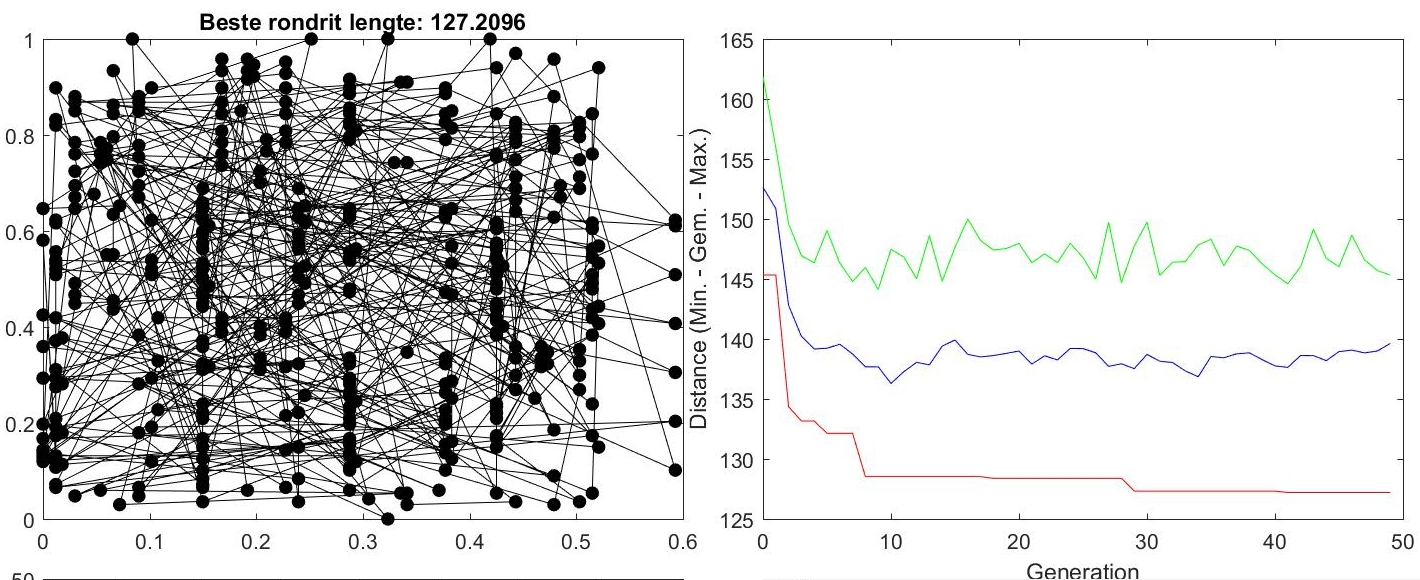
\includegraphics[width=13cm]{img/specific/order_crossover/general_1.jpg}
\end{center}

And, the best result obtained after modifying it, with the "best"
parameters, according to our general tests\\

\begin{center}
[1250,200,5\%,50\%,50\%]\\
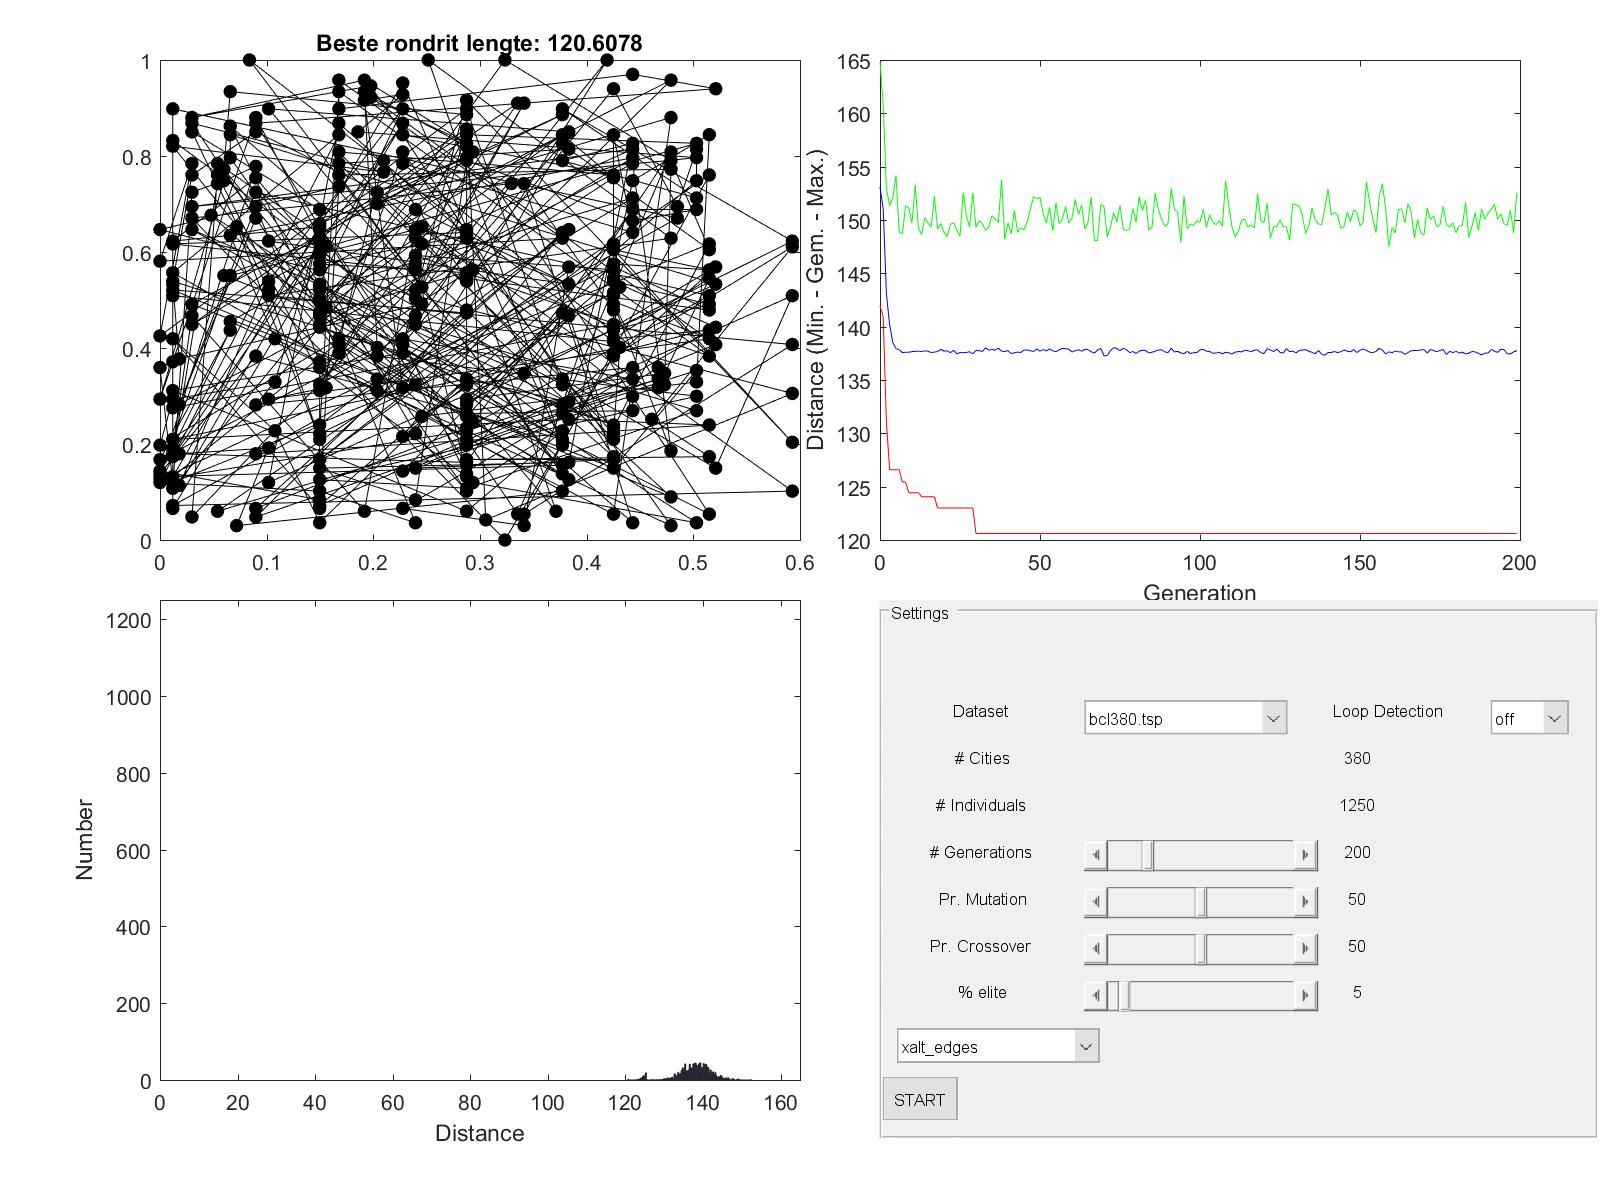
\includegraphics[width=13cm]{img/specific/order_crossover/general_8.jpg}
\end{center}

As can be seen, the new selection method started with a worse result, having
the same paramters as the base case, only with the \% of elitism
changed to the number of selected individuals, 10

\begin{center}
[50,50,10 selected,95\%,5\%]\\
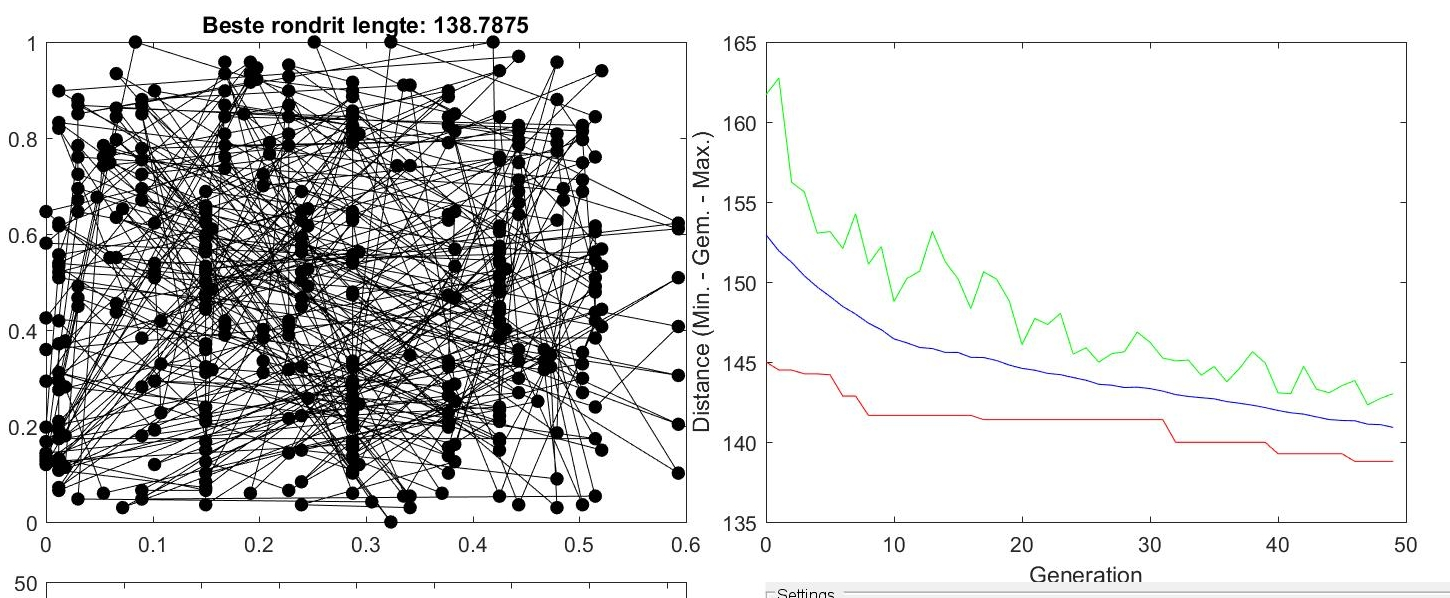
\includegraphics[width=13cm]{img/optional/optional_1.jpg}
\end{center}

The only parameter that we can test for is the number of selected
individuals from the tournament, and we did so, with 10 (the previous graph),
15,30, 45 and 50\\

\begin{center}
[50,50,15 selected,95\%,5\%]\\
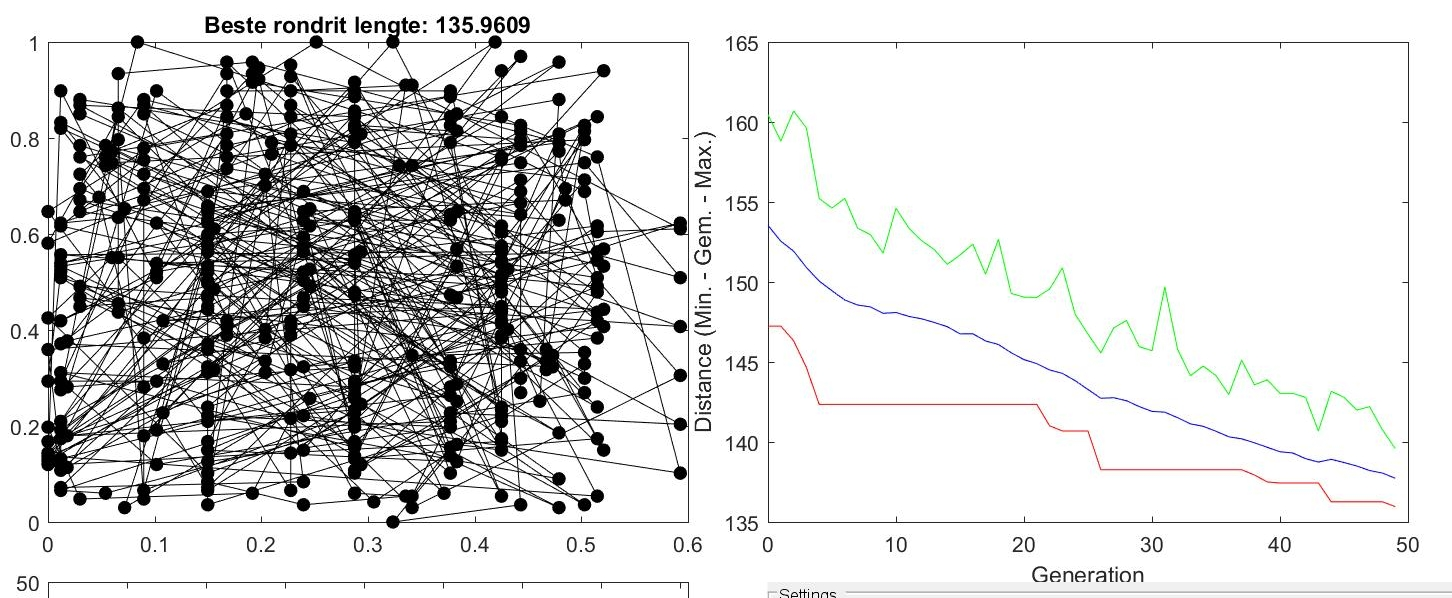
\includegraphics[width=15cm]{img/optional/optional_2.jpg}
\end{center}


\begin{center}
[50,50,30 selected,95\%,5\%\big]\\
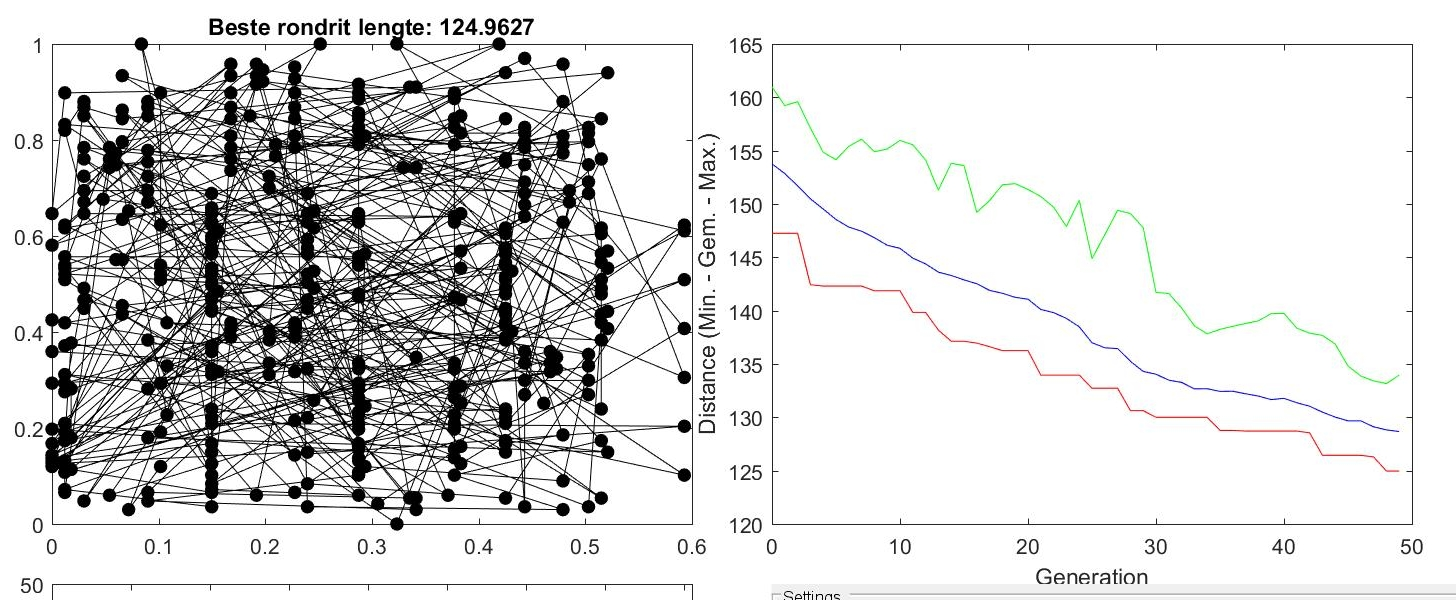
\includegraphics[width=15cm]{img/optional/optional_3.jpg}
\end{center}

\begin{center}
[50,50,45 selected,95\%,5\%]\\
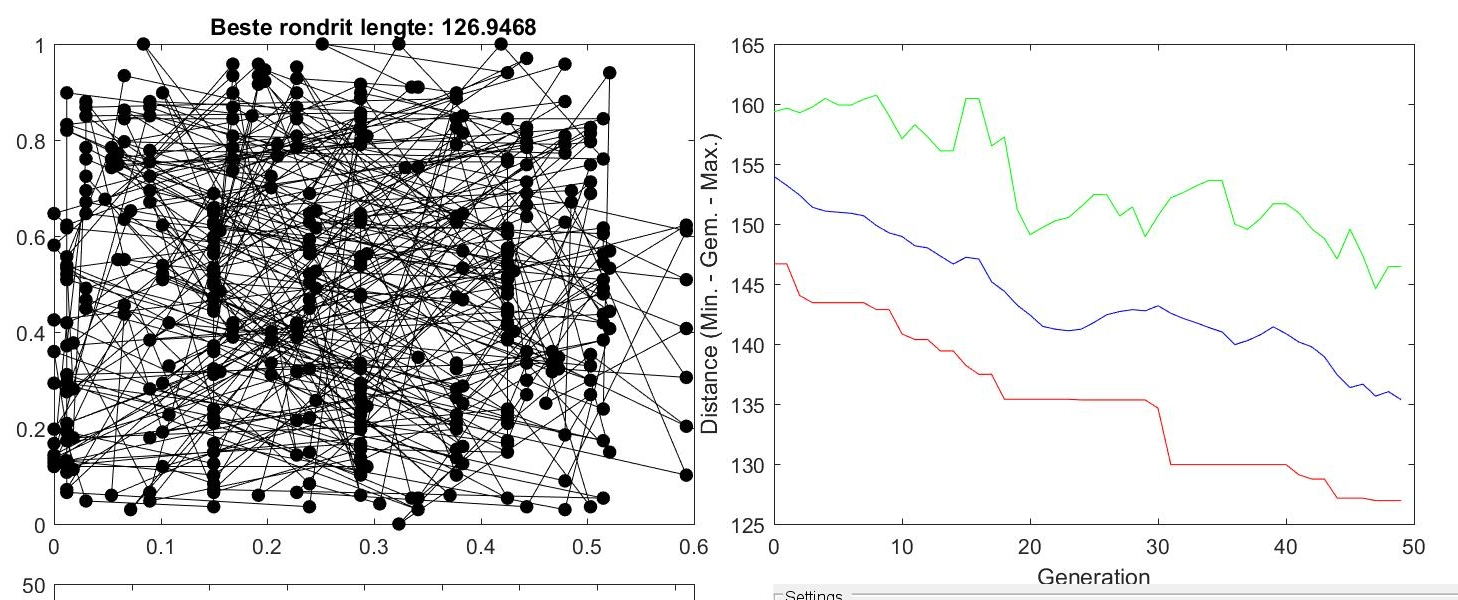
\includegraphics[width=15cm]{img/optional/optional_4.jpg}
\end{center}

\begin{center}
[50,50,50 selected\%,95\%,5\%]\\
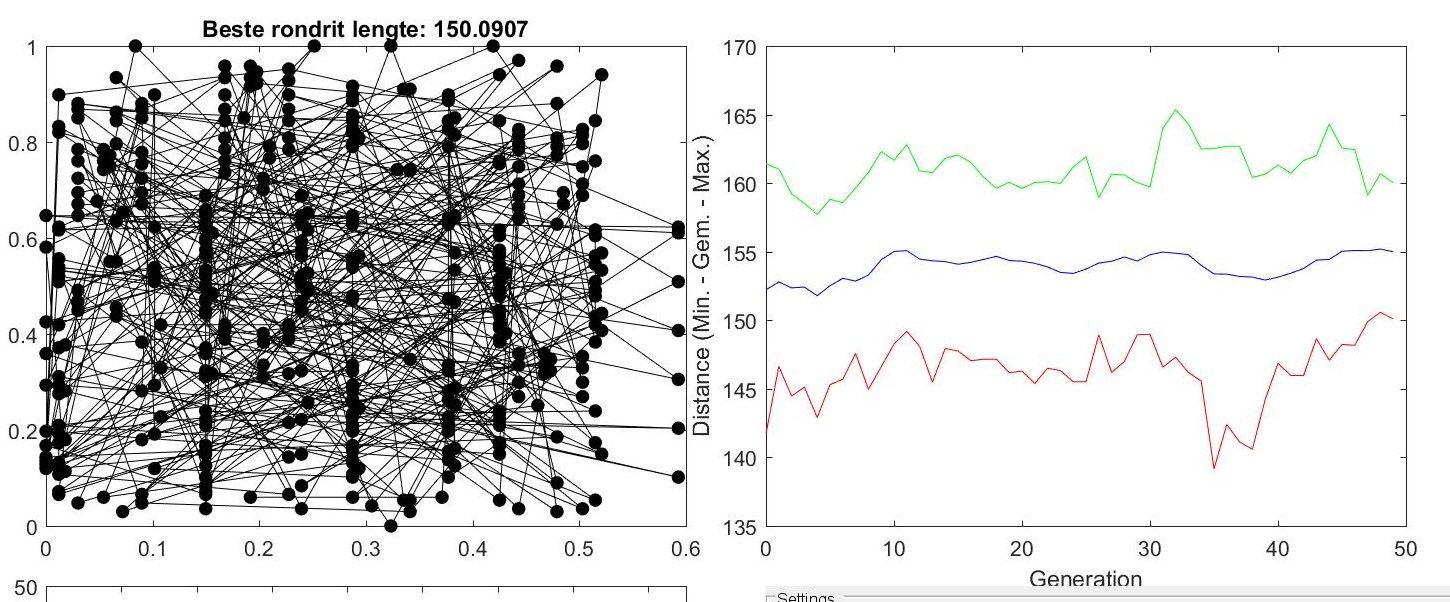
\includegraphics[width=15cm]{img/optional/optional_5.jpg}
\end{center}

As we can see, with 15 individuals the result is better, but the best outcome
comes when the number of individuals is either 30 (the best) or 45 (second
best). And, as expected, using all 50 individuals does not only not improve,
but actually worsens the result, as it modifies all individuals, no good
result is keep from generation to generation. Comparing the time spent on these
tests, around 5.5-5.8 each, it is already less time than the average of the base
case with elitism, 6.88. 
Regarding the improvement, when tuning the elitism, the result barely improved
at all, but looking at the results with this new selection method, only
modifying the number of individuals selected gives us an improvement of 9.96\%,
which is already more than the "best" solution obtained by tunning all
parameters when the selection method was elitism. It could be concluded
that this method is better for this problem.\\ 


